\documentclass[12pt, preprint]{aastex}
%\documentclass[12pt]{paper}

\newcommand{\dedalus}{\href{http://dedalus-project.org}{Dedalus}}
%\usepackage{natbib}
\usepackage[margin=1in]{geometry}
\usepackage{xcolor}
\usepackage{hyperref}
\urlstyle{same}
\hypersetup{
  colorlinks,
  linkcolor=red,
  urlcolor=olive,
  citecolor=gray
}

\title{Perspectives on Reproducibility and Sustainability of Open Source Scientific Software from Seven Years of the Dedalus Project}
\author{The Dedalus Collective}
\begin{document}
\maketitle

\section{Introduction}
\label{sec:intro}
%Background on Dedalus; mission, code, users.
As the Science Mission Directorate considers establishing an open code policy, we consider it timely to share our experiences as the developers of the open source partial differential equation solver \dedalus{}. \dedalus{} is a flexible framework for solving partial differential equations. Its development team primarily uses it for studying stellar and planetary astrophysics. While \dedalus{} was developed originally for astrophysical fluid dynamics (AFD), though it has found a much broader user base, including applied mathematicians, plasma physicists, and oceanographers. Here, we will focus on issues related to open source software from the perspective of AFD. We use the term AFD with the understanding that astrophysics simulations are inherently multi-physics: fluid dynamics coupled with some combination of gravitational dynamics, radiation transfer, relativity, and magnetic fields. This leads to very large simulation codebases, which are typically dominated by a few well-known open-source packages. However, we will argue that an open-code policy should encompass not just these large simulation codes, but also the input files and analysis scripts. \textbf{It is our interest that NASA adopt an open-code policy because without it, reproducibility in computational science is needlessly hampered.} 

With the caveat that we have not performed bibliometric analyses, it seems reasonable to assert that the majority of papers published in AFD are done using open source codes, especially in star formation, accretion disk physics, and large-scale structure formation. \emph{Athena}, \emph{Enzo}, \emph{Pencil Code}, \emph{Pluto}, and \emph{Gadget 2} are very widely used. In stellar astrophysical fluid dynamics, there are fewer examples of open-source tools, with \href{http://magic-sph.github.io}{MagIC} and \href{http://amrex-astro.github.io/MAESTRO/}{MAESTRO} as important exceptions. For many of these simulation codes, the preferred method of in-depth data analysis is via \href{http://yt-project.org}{yt}, a pioneering open-source project that introduced many of the important development and community-building concepts we use in \dedalus{}. 

\dedalus{} is written primarily in python; it has a very small code base of approximately 7000 source lines of code (SLOC)\footnote{source lines of code measured using the the \href{https://github.com/bytbox/sloc}{sloc tool} on publically available repositories of each code as of 3 January 2018}. It originated in an effort by one of us to develop a easily modifiable, modern fluid dynamics solver for studying magnetohydrodynamic turbulence problems in AFD. The first commit to the project was in 2010. In 2012, the project expanded from two people to five. Since then, nine people have made commits to the code base, including four not affiliated with the core development team. We have logged 46 pull requests, representing peer-reviewed code contributions. The code is licensed under the GNU General Public License Version 3 (GPL). We chose this license because we want to ensure that the source code always be available for inspection and auditing by any interested parties. 

We do not ask users to register before receiving the code. Doing so would, in our view, constitute a barrier to access without providing any substantive estimate on the number of users. Instead, we can estimate the size of our community by a number of metrics. We have 177 unique users participating in the \texttt{dedalus-users} mailing list, and 13 unique users participating in the \texttt{dedalus-dev} mailing list for developers. Dedalus has been used in at least thirteen peer-reviewed publications \citep{2017PhRvF...2h3501A,PhysRevFluids.2.094804,2017ApJ...841....1C,2017ApJ...841....2C,2017MNRAS.466.2181L,2016ApJ...832...71L,2016JCoPh.325...53V,2016PhRvE..94e3206D,2016PhRvL.116j5004D,2016MNRAS.455.4274L,2015PhRvE..91f3016L,2014ApJ...797...94L}.

The subcommunity of astrophysical fluid dynamics modelling thus tends to embrace open-source even without an official policy. However, this is, in our view, not sufficient, especially as it can vary from field to field: many of the most important spherical dynamo codes for studying stellar and planetary magnetic fields remain closed-source (e.g. \emph{Rayleigh}, \emph{ASH}, various derivatives of the Glatzmaier/Gilman code). The simulation code is only one part of a long pipeline that starts with an idea and ends with a published result. An open-code mandate should eliminate any closed-source bottlenecks that could hamper what is, in our view, the cornerstone of the scientific computing enterprise: repeatability. That is, simply because the largest piece of software is available, if the input files and analysis scripts are not also public, reproducibility becomes impossible. 

These codes tend to be very large: Athena has $\simeq 80,000$ SLOC; Enzo is over $120,000$ lines! 

Here, we argue that the benefits of open-source projects far exceeds their costs; we outline our view on exactly what those benefits and costs are, and we suggest that in order to maximize scientific returns on software development, \emph{open-source} is not enough. The best use comes from \emph{community-driven} software tools that blur lines between users and developers. Nevertheless, we strongly recommend that Science Mission Directorate adapt an open code policy that embraces \emph{explicitly licensed}, discoverable software. 

\section{Reproducibility}
\label{sec:repro}

Two of the most important tasks in computational modelling are \textbf{verification} and \textbf{validation}. In the context of numerical simulation, verification is the assessment of ensuring the software correctly solves a given set of equations; validation is the act of ensuring the equations solved correctly reproduce the physical phenomena of interest \citep{2002PrAeS..38..209O}. 

Open source tools strongly facilitate this activity. Verification tests are plentiful; there is a strong tradition of benchmark problems and inter-code comparisons in AFD \citep[e.g.][among many others]{2001JGR...106.3715B,2014GeoJI.197..119M,2014ApJS..210...14K,2016MNRAS.455.4274L}.

In particular, validation is nearly impossible for astrophysical fluid dynamics when applied directly to the problems of interest: there are precious few astrophysical experiments that can be done repeatably in the lab. Outside of direct astrophysical problems, one could perform validation tests against known terrestrial fluid dynamics problems.  However, many such flows involve complex boundary layers, which are rare enough in astrophysics to often be excluded from many AFD codes. 

There are several important ways in which we can attempt validation. NASA has already developed a set of best practices for verification and validation computational fluid dynamics (\url{https://www.grc.nasa.gov/www/wind/valid/tutorial/valassess.html}). 

\section{Maintenance and User Support}
\label{sec:support}

% What are the additional burdens placed on developers because of open source? A difficult question to answer directly, but can come at this obliquely by thinking about the \emph{total amount of time} we spend answering user questions. How does this burden the developers? What \emph{rewards} if any does doing this kind of support do? Do we understand the code better because of it (think of wave-driving example)? 

Providing open-source code is not without cost. Direct costs are quite minimal; they are limited to web hosting. The source for \dedalus{} is hosted at \href{https://bitbucket.org}{Bitbucket}, a commercial provider of distributed version control services that allows open source projects to be hosted for free. An often-discussed cost of open-source research products is the ``need'' to provide user support for them. However, we have found that, despite supporting a user base across many scientific disciplines, the amount of direct user support we do is small. Indirect user support, in the form of responding to bug reports and implementing enhancements suggested by users is also small, amounting to no more than a few person hours per month. Figure~\ref{fig:messages} shows the number of messages per month sent to the the two mailing lists we maintain, \texttt{dedalus-users} for discussions of using the code and \texttt{dedalus-dev} for discussions of development of new features. The users list shows a steady (roughly linear) average growth over the past two and a half years, with a peak of just over 80 messages in one month. Making a rough assessment of 15 minutes per message, this represents approximately 10 person-hours per month on the part of the developers, if we assume that half of the messages are questions and the other half responses. Given a development team of 5, this represents an upper limit of 2 hours per month per developer. However, we note that members of our user community often \emph{answers} questions on this list in addition to asking them (and developers also \emph{ask} questions too!). The groups themselves are archived and searchable, making them a knowledgebase for users. 

\begin{figure}
  \centering
  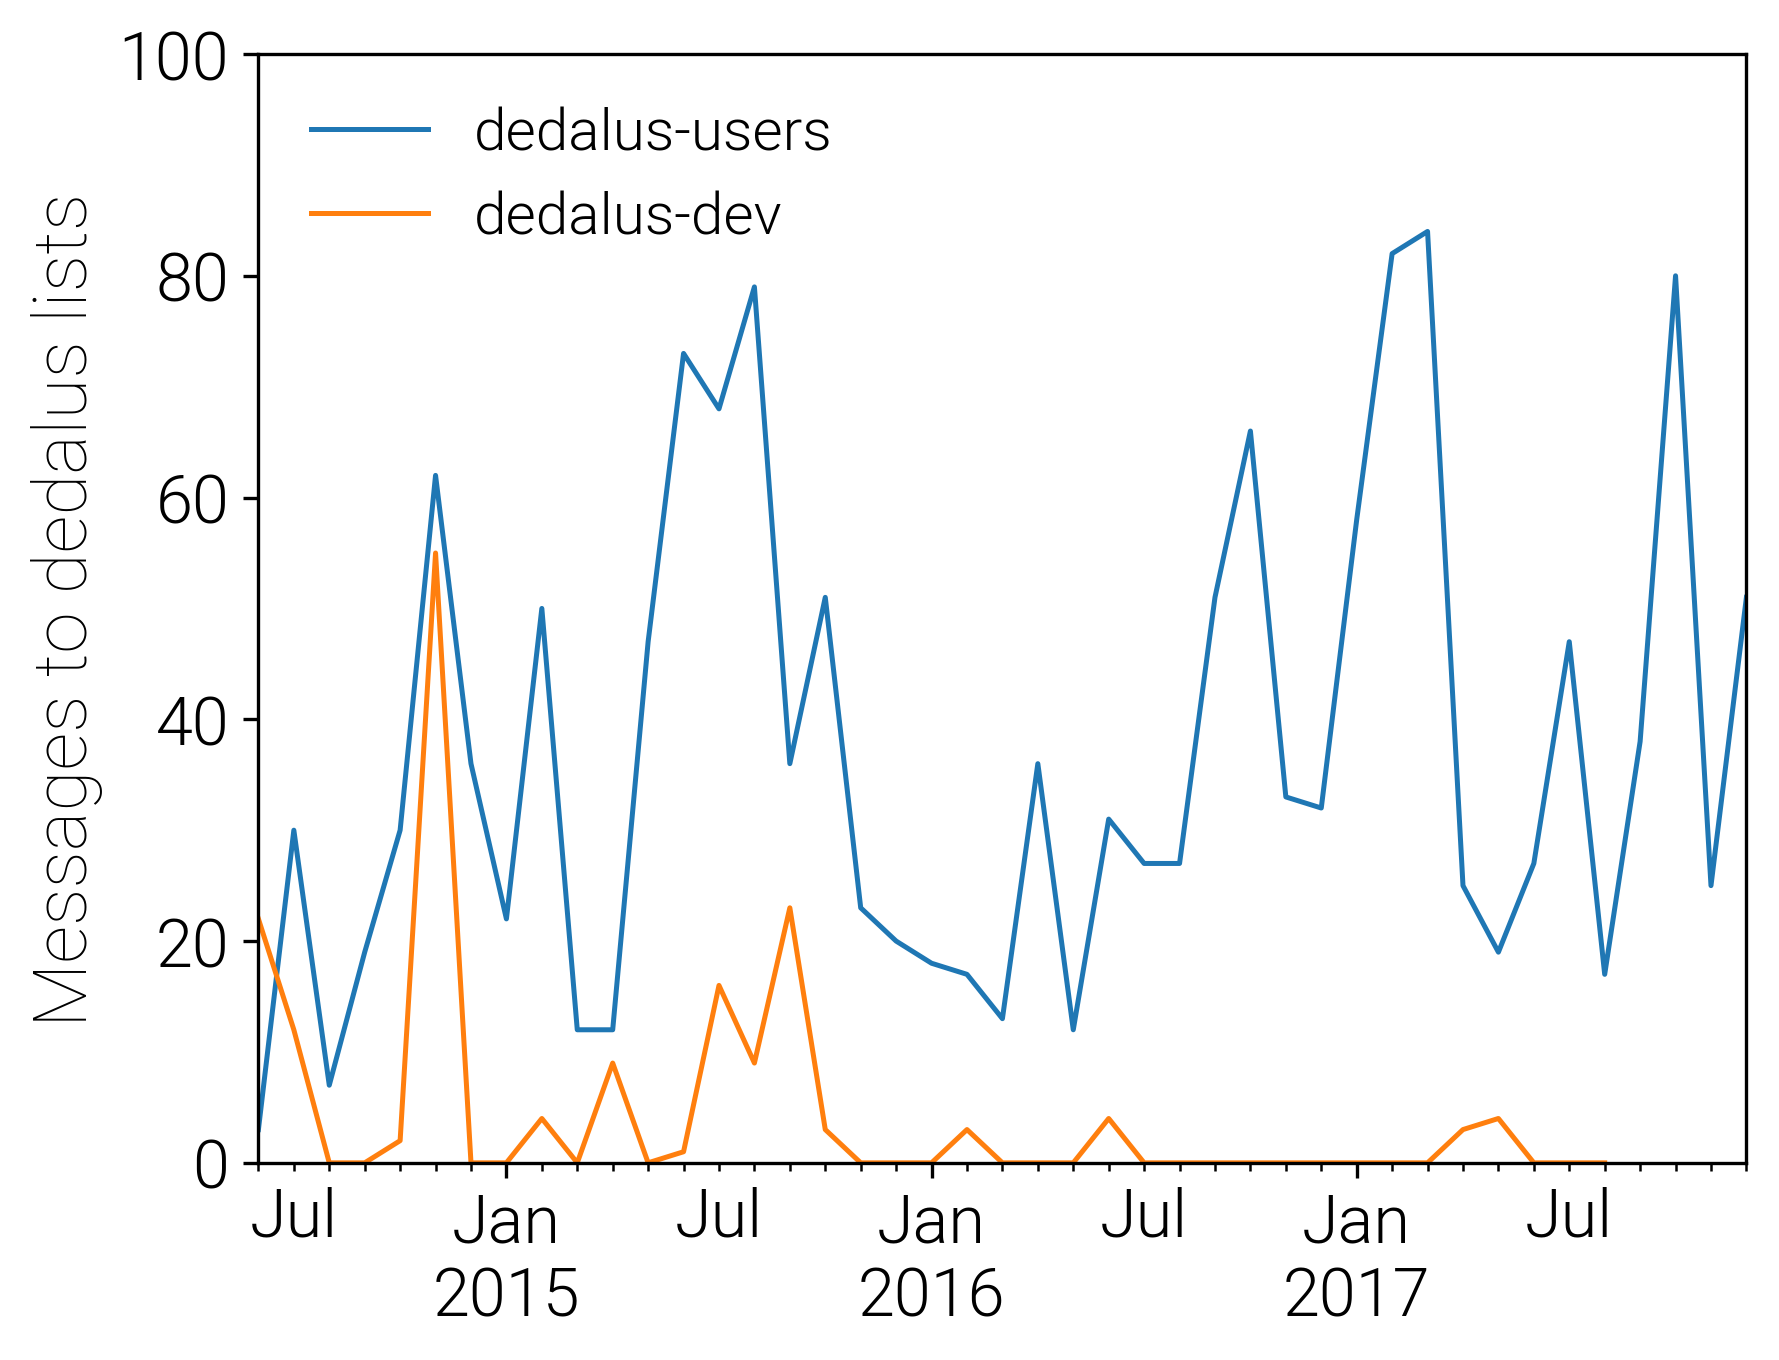
\includegraphics{../figs/message_counts.png}
  \caption{Message traffic on the \texttt{dedalus-users} and \texttt{dedalus-dev} google groups.}
  \label{fig:messages}
\end{figure}

\section{Software stack}
\label{sec:stack}

The use of a completely open source stack/toolchain (we need to avoid too many buzzwords here) significantly affects the workflow, for both good and bad. On the good side, we are encouraged to tap into a very large infrastructure of open source things (jupyter, docker, possible cocalc integration) that can blend research at many scales (simple 1D things running in the cloud/on a laptop all the way to supercomputing) and education. On the bad side, installation is a nightmare; something that open source communities often do not focus on enough.

\section{Looking to the Future}
\label{sec:future}

Containerizing applications; stack dependence; installation; ensuring supercomputing facilities are up-to-date on this.
\appendix

\section{Supporters}
\label{sec:supporters}

``A numbered list of supporters who did not contribute significantly to the text'' goes here.

\bibliographystyle{apj_title}
\bibliography{dedalus}

\end{document}
